%%%%%%%%%%%%%%%%%%%%%%%%%%%%%%%%%%%%%%%%%%%
\subsection{Результаты работы}
%%%%%%%%%%%%%%%%%%%%%%%%%%%%%%%%%%%%%%%%%%%
\begin{frame}%[allowframebreaks=0.9,t]

    Компилятор Kodept является консольным приложением, поэтому для него был разработан интерфейс командной строки (CLI).
    С помощью него можно настроить вид выходных данных, поведение работы и др.
    Кроме того, можно получить внутреннюю модель в виде графа.
    Для этого следует использовать следующую команду (рис. \ref{fig:ast_dot}):

    \begin{center}
        \texttt{./kodept graph examples/test.kd}
    \end{center}

    Для демонстрации работы механизма вывода типов можно использовать следующее:

    \begin{center}
        \texttt{./kodept -d examples/test.kd}
    \end{center}

    В таком случае тип функции \lstinline{compose} будет таким:

    \begin{center}
        \texttt{[compose: $\forall a, b, c => ('b -> 'a) -> ('c -> 'b) -> 'c -> 'a$]}
    \end{center}

    \vspace{0.5cm}

    Проект можно развивать и дальше - улучшая как саму работу механизма, так и добавляя другие функции, например этап компиляции.

\end{frame}

\begin{frame}
    \begin{figure}[H]
        \centering
        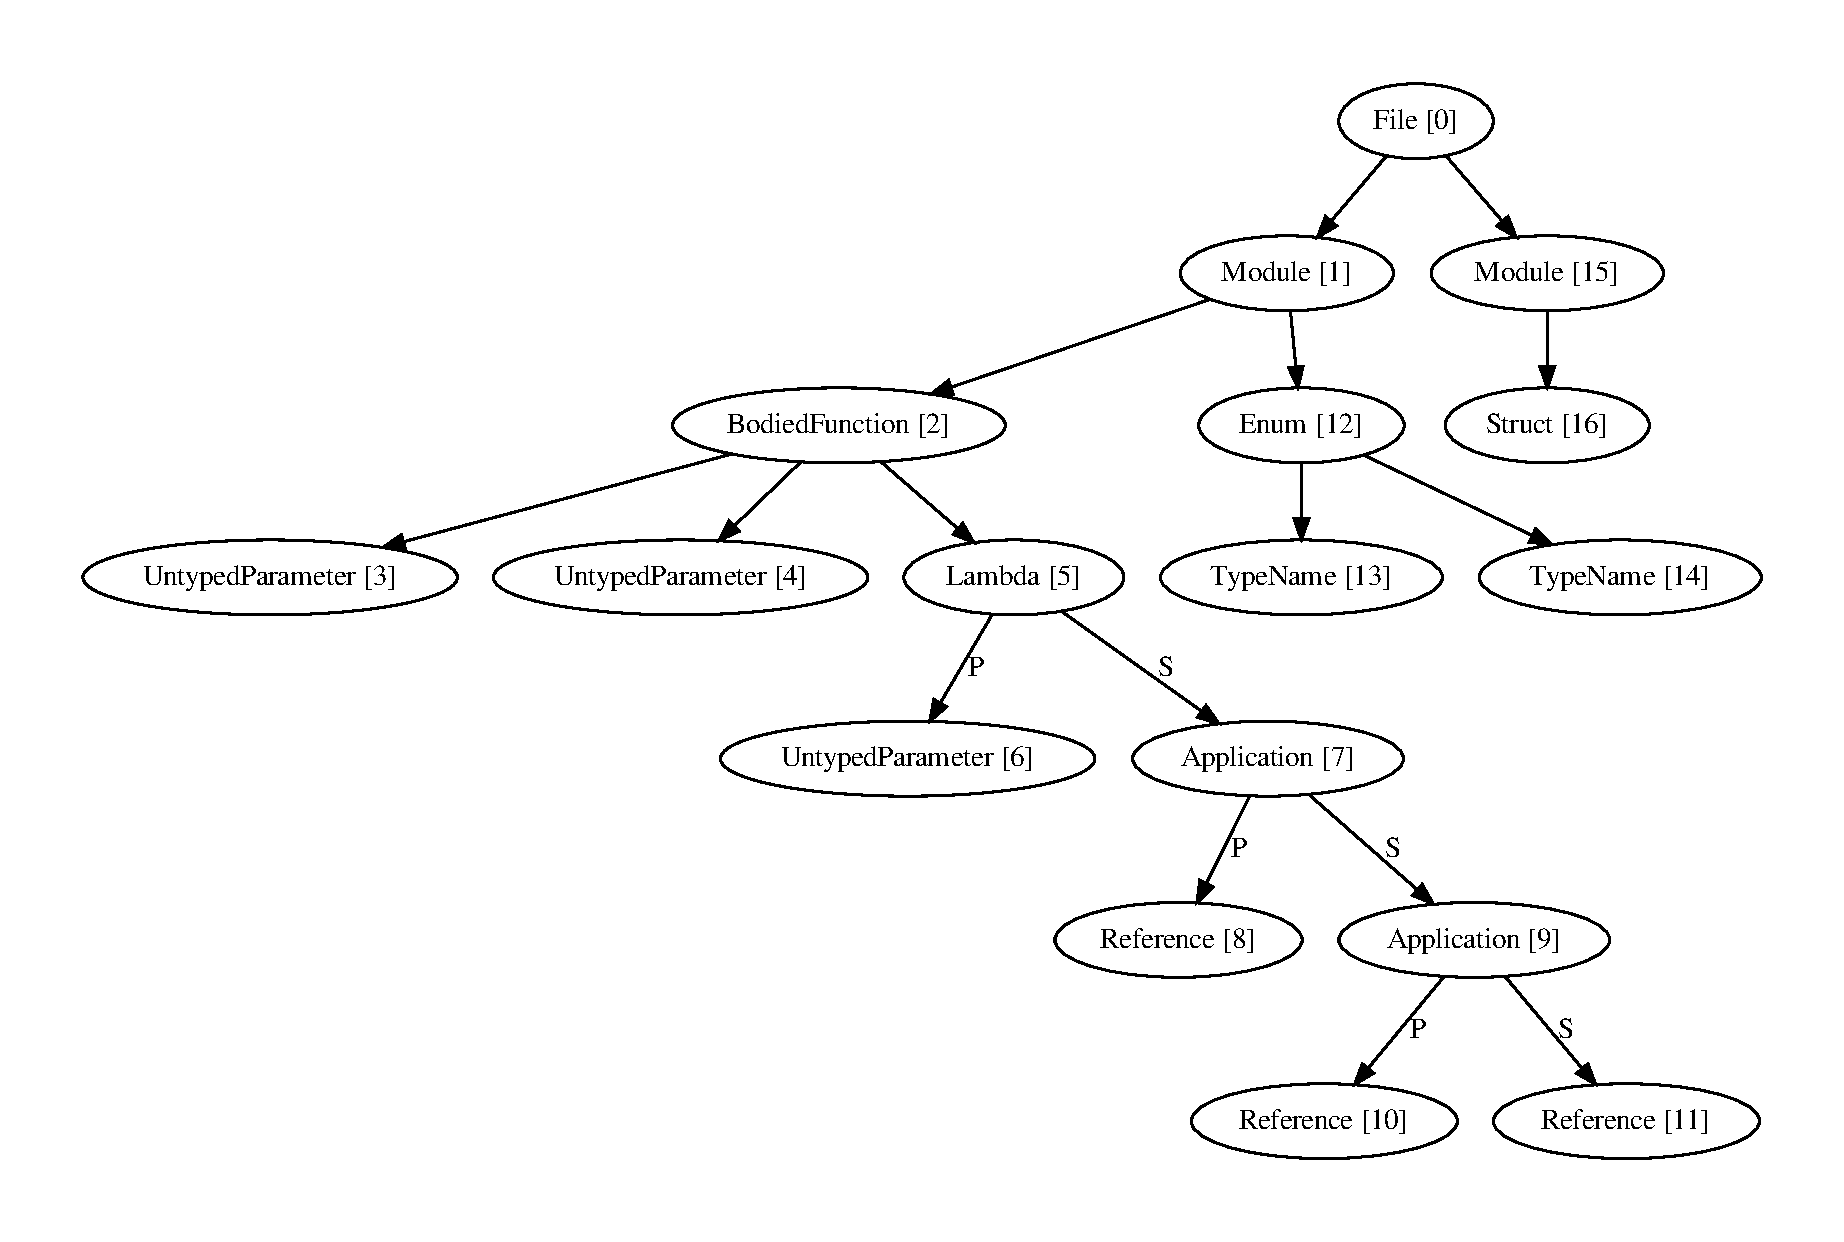
\includegraphics[height=0.8\textheight]{figures/dot}
        \caption{Изображение структуры абстрактного синтаксического дерева}
        \label{fig:ast_dot}
    \end{figure}
\end{frame}
%%%%%%%%%%%%%%%%%%%%%%%%%%%%%%%%%%%%%%%%%%%
